\documentclass{ccn}

\addbibresource{bib/references.bib}

\usepackage{graphicx}
\usepackage{booktabs}
\usepackage{subcaption}
\usepackage{dblfloatfix}
\usepackage{placeins}

% Compact but stable float behavior for two-column layout.
\setcounter{topnumber}{3}
\setcounter{dbltopnumber}{2}
\setcounter{bottomnumber}{2}
\setcounter{totalnumber}{5}
\renewcommand{\topfraction}{0.95}
\renewcommand{\dbltopfraction}{0.95}
\renewcommand{\bottomfraction}{0.5}
\renewcommand{\textfraction}{0.05}
\renewcommand{\floatpagefraction}{0.85}
\renewcommand{\dblfloatpagefraction}{0.85}
\setlength{\textfloatsep}{6pt plus 2pt minus 2pt}
\setlength{\dbltextfloatsep}{6pt plus 2pt minus 2pt}
\setlength{\floatsep}{4pt plus 2pt minus 2pt}
\setlength{\dblfloatsep}{4pt plus 2pt minus 2pt}
\setlength{\intextsep}{4pt plus 2pt minus 2pt}
\setlength{\abovecaptionskip}{3pt}
\setlength{\belowcaptionskip}{0pt}

% Avoid vertical centering on float-only pages (removes large top whitespace).
\makeatletter
\setlength{\@fptop}{0pt}
\setlength{\@dblfptop}{0pt}
\makeatother

\title{Neural Similarity Patterns Support a Categorical Boundary Between 4 and 5 in Numerosity (1-6)}
\author{}

\begin{document}
%\linenumbers

\maketitle

\begin{abstract}
Non-symbolic numerical cognition has been explained by either a single continuous magnitude code or dual representational systems: Parallel Individuation (PI) for small exact sets and the Approximate Number System (ANS) for larger approximate sets. We tested these accounts in 24 adults using single-trial EEG during an oddball change-detection task with dot arrays from 1 to 6. We computed whole-epoch and time-resolved representational dissimilarity matrices and compared them with ANS and PI boundary models at 3-4 and 4-5. With all numerosities included, ANS fits were strong and distance effects were pronounced. After excluding numerosity 1, ANS fits were attenuated while PI boundary structure was preserved. In the no-1 whole-epoch analysis, the Target PI(2-4) model outperformed Target PI(2-3) ($d = 0.79$, $p < 0.001$). Time-resolved model-difference tests also favored the 4-5 boundary across multiple windows. These findings support a dual-system account and place the PI capacity boundary at 4-5 in adults, while also showing that numerosity 1 is a distinct case that can increase the estimated fit of a single continuous magnitude code.
\end{abstract}

\section{Introduction}
Small sets of objects (typically 1-3, sometimes up to 4) are enumerated rapidly and precisely, a phenomenon known as subitizing, while larger sets require estimation that follows Weber's law. One account explains this pattern through a single continuous magnitude code with scalar variability across the entire numerical range \citep{GallistelGelman2000}. Under this single-system view, small-number advantages reflect higher resolution at the low end of a continuous scale. An alternative account proposes two distinct representational systems: Parallel Individuation (PI), which tracks small sets of discrete items through ``object files'' and is often linked to subitizing, and the Approximate Number System (ANS), which represents larger quantities as noisy magnitude estimates with ratio-dependent discriminability \citep{FeigensonCarey2003,FeigensonDehaeneSpelke2004}.

These accounts make distinct predictions about neural similarity
structure. If numerosity is represented by a single continuous code, neural
similarity should scale with numerical ratio with no categorical
boundary. If PI and ANS are distinct, a categorical break should
separate their ranges at the PI capacity limit. The subitizing range
is often described as approximately 1-4 items \citep{TrickPylyshyn1994},
though reported limits vary across tasks and individuals
\citep{Cowan2001}, placing the
predicted boundary at either 3-4 or 4-5.

Neural similarity analysis can test which boundary model better captures
the representational structure. Representational similarity analysis
\citep[RSA;][]{Kriegeskorte2008} compares neural representational
dissimilarity matrices (RDMs) to model predictions. We apply
time-resolved RSA to single-trial EEG from 24 adults performing an
oddball change-detection task with 1-6 dot arrays. Using Linear
Discriminant Analysis (LDA) classifiers, which capture multivariate
spatiotemporal patterns from the EEG signal
\citep{KingDehaene2014}, we construct whole-epoch target RDMs
(6$\times$6) and 24-condition prime-target RDMs, comparing them against
PI models with boundaries at 3-4 and 4-5, a graded ANS model, and
reaction-time and pixel controls.

A complication in testing these predictions is the special status of
numerosity~1. Under Weber-law scaling, ``1'' is maximally distant from
all larger numerosities (the log-ratio between 1 and any other
numerosity is the largest possible), which can inflate ANS model fits. In addition,
numerosity~1 may be categorically privileged via a
singular-versus-plural (one-vs-more-than-one) distinction
\citep{Barner2007,Barner2008,Li2009}. To disentangle these effects, we
repeat all analyses after excluding pairs containing numerosity~1.

Across analyses, the data favor a dual-system account over a single
continuous magnitude code. ANS-like fits are strongest when numerosity~1
is included, but excluding ``1'' attenuates ANS fits while preserving PI
boundary structure. The 4-5 boundary outperforms the 3-4 alternative,
suggesting PI capacity at four items. Numerosity~1 is a distinct case
whose inclusion can increase the estimated fit of continuous models.

\section{Methods}

\subsection{Participants and Task}
Twenty-four adults (mean age 27.31 years) performed a numerical
change-detection task using an oddball paradigm with dot-array stimuli
representing quantities 1-6. EEG was recorded continuously at 250 Hz
from a 128-channel EGI HydroCel Geodesic Sensor Net.
Each trial consisted of 3-5 ``prime'' images of the same numerosity
(250 ms each, jittered ISI of 750-1250 ms), followed by a target
image. On change trials, the target differed from the prime and
participants pressed a button to indicate they detected a change.
Each change trial is defined by its prime-target pair. For example,
a trial with prime 4 and target 2 is coded as condition ``42.''
Prime and target always differ by at most 3 items within the 1-6
range, yielding 24 unique prime-target conditions
(Figure~\ref{fig:task-design}). We analyzed all change trials
(both correct and incorrect responses), resulting in 216 usable
epochs per participant (9 trials per condition per participant).

\begin{figure}[!t]
  \centering
  \begin{minipage}[t]{\columnwidth}
    \centering
    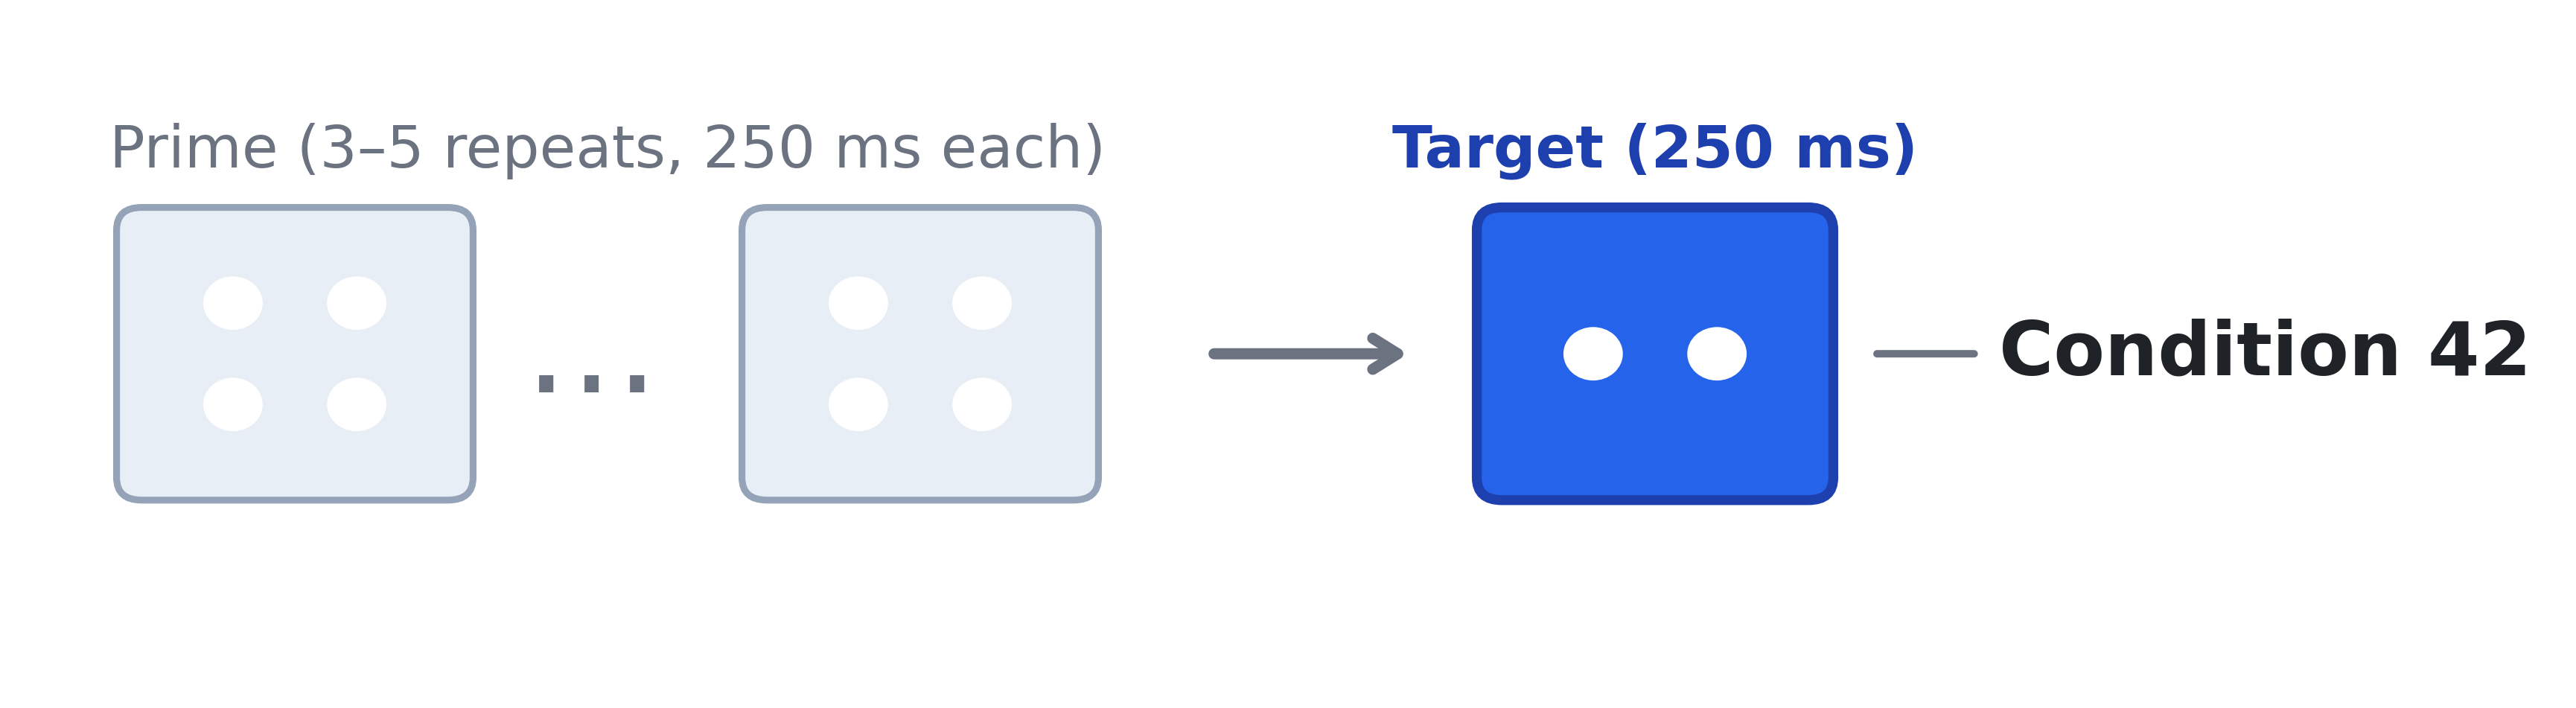
\includegraphics[width=0.85\columnwidth]{media/trial_structure.png}
    \vspace{-1mm}
    \subcaption{Single-trial structure. Three to five identical prime
    images precede a target that differs in numerosity. Condition codes
    denote the prime-target pair (e.g., ``42'' = prime 4, target 2).}
    \label{fig:trial-structure}
  \end{minipage}

  \vspace{4pt}

  \begin{minipage}[t]{\columnwidth}
    \centering
    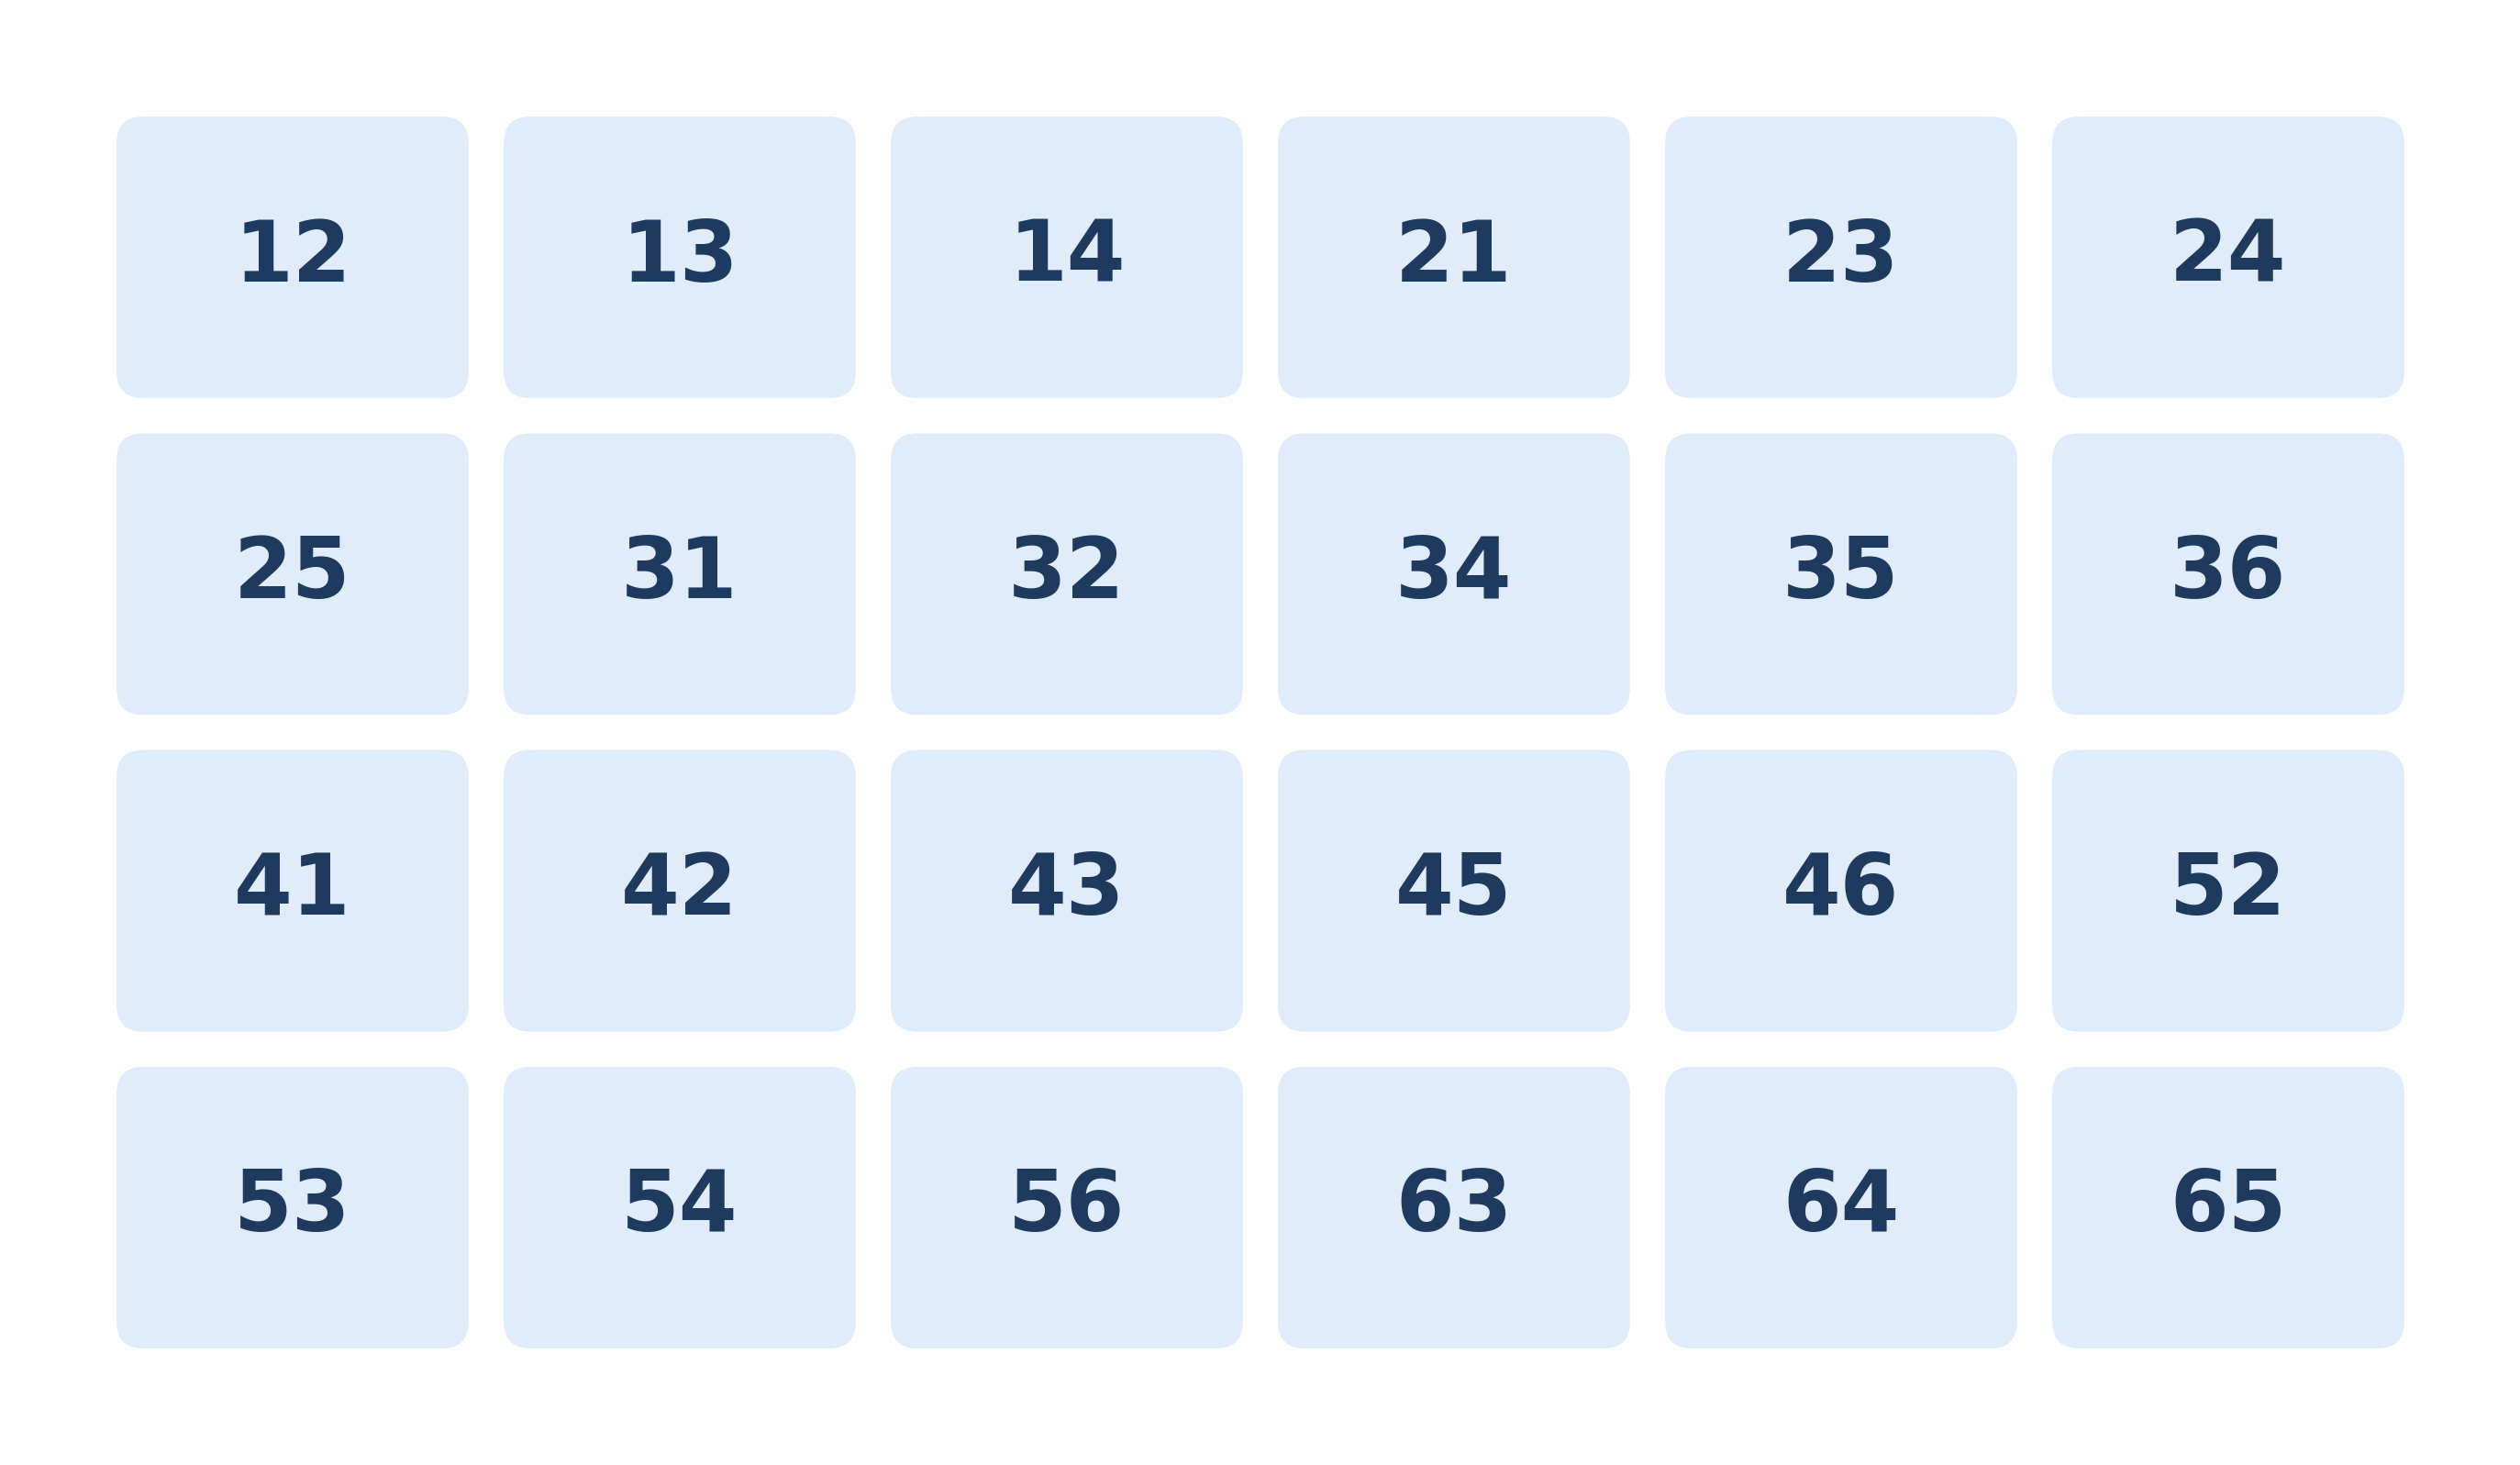
\includegraphics[width=0.75\columnwidth]{media/conditions-24.png}
    \vspace{-1mm}
    \subcaption{All 24 prime-target change conditions used in this
    study. Prime and target differ by 1-3 items within the 1-6 range.}
    \label{fig:condition-matrix}
  \end{minipage}

  \vspace{4pt}

  \begin{minipage}[t]{\columnwidth}
    \centering
    
\includegraphics[width=0.70\columnwidth]{media/conditions-6.png}
    \vspace{-1mm}
    \subcaption{Whole-epoch target numerosities (1-6), obtained by
    collapsing across prime identity in (b).}
    \label{fig:condition-6}
  \end{minipage}
  \caption{Task design.}
  \label{fig:task-design}
\end{figure}


\subsection{Preprocessing}
EEG data were preprocessed using the Harvard Automated Processing Pipeline
for Electroencephalography \citep[HAPPE v4.1.0;][]{GabardDurnam2018HAPPE}.
Preprocessing included a 1.5-35 Hz bandpass filter and 60 Hz line-noise
removal (CleanLine). HAPPE identified and interpolated bad
channels and applied wavelet-based artifact correction (soft
thresholding).
Each epoch was baseline-corrected using the prestimulus interval
(-200 to 0 ms).

\subsection{Representational Similarity Analysis}
We used Representational Similarity Analysis (RSA) to compare neural
and theoretical dissimilarity structures \citep{Kriegeskorte2008}.
For each pair of conditions, we trained a classifier to discriminate
the two conditions and used the resulting binary decoding accuracies to construct
a neural representational dissimilarity matrix (RDM). We then correlated these neural RDMs with
theoretical model RDMs encoding competing hypotheses about numerosity
representation.

We used Linear Discriminant Analysis (LDA) with Ledoit-Wolf
regularization (scikit-learn, \citealp{Pedregosa2011}) for binary
numerosity classification. To prevent data leakage
\citep{KapoorNarayanan2023Leakage}, we used subject-wise GroupKFold
cross-validation (6 folds), so that no subject appeared in both
training and test sets within a fold. Cluster-based permutation tests
used MNE-Python \citep{Gramfort2013}.

\subsection{Theoretical Model RDMs}
The following theoretical RDMs encode competing hypotheses about the
representational structure of numerosity and serve as predictions
for whole-epoch and temporal analyses
(Figures~\ref{fig:static-model-rdms} and~\ref{fig:temporal-change24-model-rdms}).
\begin{itemize}
  \item \textbf{Target PI}: A family of models encoding the target's
    system membership. Numerosities at
    or below a boundary $B$ are assigned to PI, and those above $B$ to
    ANS. Within PI, dissimilarity is a fixed constant (categorical).
    Within ANS, dissimilarity follows $|\log(a/b)|$. Cross-system
    pairs receive an elevated baseline plus log-ratio scaling:
    $d = c + |\log(a/b)|$, where $c$ is a boundary constant. We
    tested two boundary locations ($B = 4$ and $B = 3$) crossed with
    two numerosity ranges (1-6 and 2-6), yielding four variants:
    Target PI(1-4), Target PI(1-3), Target PI(2-4), and Target
    PI(2-3). The no-1 variants exclude numerosity~1 from both prime
    and target during training and evaluation.
  \item \textbf{ANS}: A graded distance model assuming a single
    continuous magnitude code with no categorical boundary.
    Dissimilarity scales with numerical ratio following Weber's law,
    $d(i,j) = |\log(a/b)|$.
  \item \textbf{Pixel}: A visual control model, included because
    dot-array stimuli covary with low-level properties such as total
    area and density.
    $d(i,j) = |\text{area}_i - \text{area}_j|$,
    the absolute difference in total white-pixel area between the two
    stimulus images.
  \item \textbf{RT}: A behavioral-difficulty control model.
    $d(i,j) = |\overline{\text{RT}}_i -
    \overline{\text{RT}}_j|$, the absolute difference in grand-mean
    reaction time between conditions. RTs were computed from correct
    trials only, winsorized at the 2.5th and 97.5th percentiles within
    each subject and condition, then averaged across subjects.
\end{itemize}

\begin{figure*}[!t]
  \centering
  \begin{minipage}{\textwidth}
    \centering
    \textbf{(a)} Target-only analysis (numerosities 1-6)\par\smallskip
    \includegraphics[width=\textwidth]{../results/analysis-lda/static-change6/static_change6_all/figures-pairwise/temporal_model_rdms_all_compact_row-static_change6_all-pairwise.png}
  \end{minipage}
  \vspace{4pt}
  \begin{minipage}{\textwidth}
    \centering
    \textbf{(b)} Target-only no-1 analysis (numerosities 2-6)\par\smallskip
    \includegraphics[width=\textwidth]{../results/analysis-lda/static-change5/static_change5_all/figures-pairwise/temporal_model_rdms_all_compact_row-static_change5_all-pairwise.png}
  \end{minipage}
  \caption{Brain and model RDMs (0-700 ms). Brain RDMs show mean
  balanced accuracy (\%) across subjects. Model RDMs show predicted
  dissimilarity for each theoretical model. The RT model shows absolute
  differences in grand-mean reaction time. The Pixel model shows
  absolute differences in white-pixel area. In this stimulus set, total
  area is similar within numerosities 1-3 and within 4-6 but drops
  sharply between 3 and 4, so the Pixel model's largest discontinuity
  falls at 3-4. (a)~Target numerosities 1-6. Pairs involving
  numerosity~1 show the highest discriminability, giving the brain RDM
  an ANS-like gradient dominated by distance from~1
  (Table~\ref{tab:static-model-comparison}). In the boundary region,
  pairs 4-5 and 4-6 show slightly higher discriminability than pairs 2-4
  and 3-4, consistent with a boundary at 4-5 rather than 3-4.
  (b)~Target numerosities 2-6 (numerosity~1 excluded from both prime and
  target during training and evaluation). With numerosity~1 removed, the
  boundary structure becomes clearer. Pairs crossing the 4-5 boundary
  (4-5, 4-6) show higher discriminability than pairs within the PI range
  (2-4, 3-4), matching the Target PI(2-4) prediction
  (Table~\ref{tab:static-model-comparison}). The Pixel model predicts
  the opposite pattern, with highest dissimilarity across the 3-4
  boundary, and does not reach significance
  (Table~\ref{tab:static-model-comparison}).}
  \label{fig:static-model-rdms}
\end{figure*}


We used a two-part analysis strategy to balance sensitivity to stable
representational structure and temporal resolution. The whole-epoch
analysis tests whether a target numerosity structure is present when
evidence is aggregated across the post-stimulus interval. The temporal
analysis tests how numerosity-related structure evolves over time using
time-resolved neural RDMs that preserve prime-target condition
identity.

\subsection{Whole-Epoch Target RSA}
The whole-epoch analysis collapses across prime identity, retaining
only the target numerosity (Figure~\ref{fig:condition-6}). LDA classifiers discriminated between
target numerosities over a 0-700 ms post-stimulus epoch (no sliding
window), producing a single RDM per subject. This analysis
has two variants: the target-only analysis (numerosities 1-6) and the
target-only no-1 analysis (numerosities 2-6), which excludes
numerosity~1 from both prime and target during classifier training
and evaluation. This no-1 variant isolates boundary structure in the
2-6 range by separating it from effects specific to numerosity~1.

\subsection{Temporal RSA}
Sliding-window RSA (50 ms window, 20 ms stride) used window
centers from $-100$ to 700 ms relative to target onset (first
window: $-125$ to $-75$ ms, centered at $-100$ ms; subsequent windows
advanced by 20 ms), using the full 24-condition prime-target structure
(Figure~\ref{fig:condition-matrix}). Each time window produces a
24 $\times$ 24 RDM that preserves the identity of both prime and
target. For the no-1 control, pairs containing numerosity~1 are
excluded from the existing RDM,
reducing the matrix to 18 $\times$ 18.

\subsection{Statistics}
Spearman correlation ($\rho$) quantified model-brain similarity, and
multidimensional scaling (MDS) visualized representational geometry
\citep{Kriegeskorte2008}. To contextualize model-fit magnitudes, we
computed a lower-bound noise ceiling using leave-one-subject-out
cross-validation: for each subject, we correlated that subject's neural
RDM with the mean RDM of all remaining subjects, then averaged across
subjects. For temporal analyses, this was computed at each time window.

For the whole-epoch analysis, one-sample $t$-tests (Holm-corrected
across models) assessed significance of Fisher-$z$-transformed
per-subject model correlations. Boundary contrasts compared Target
PI(x-4) versus Target PI(x-3) using paired $t$-tests on Fisher-$z$
differences (two-sided, Cohen's $d_z$).

For the temporal analysis, cluster-based permutation tests (5,000
permutations, $\alpha = 0.05$) identified sustained periods of
significant model-brain correlation. Cluster-forming thresholds used
the $t$-critical value with $\text{df} = N - 1$ (one-sided for
model-fit tests), with a minimum cluster size of 2 consecutive
windows. Individual decoding accuracy was tested against chance using
the same one-sided cluster-based permutation framework.

Model comparisons applied the same framework to
Fisher-$z$-transformed Spearman correlation differences at each time
window (10,000 permutations, two-sided, $\alpha = 0.05$), including
boundary-location tests (4-5 vs.\ 3-4). All analyses were repeated
with and without numerosity~1.

\section{Results}

\subsection{Distance-Dependent Decoding}
If numerosity is represented as a continuous magnitude, conditions that
are numerically farther apart should produce more distinct neural
patterns and thus higher decoding accuracy. We tested this by grouping
condition-pair decoding accuracies by the absolute difference between
the two conditions' target numerosities and computing the group mean at
each time window.
Figure~\ref{fig:temporal-distance}a shows that pairs separated by
greater numerical distance tend to be decoded more accurately, with
the clearest graded ordering by distance in early (80-200 ms) and mid-latency
(340-500 ms) windows. Across all six numerosities, this graded pattern is consistent with a
distance-dependent neural code.

\paragraph{The ``No-1'' control.}
To assess whether the distance gradient is driven by the inclusion of
numerosity~1, we repeated the analysis excluding all pairs
containing ``1'' (Figure~\ref{fig:temporal-distance}b). Sustained
separation by numerical distance largely disappears, with the clearest
residual distance-related gradient limited to approximately 80-120 ms. This suggests that
numerosity~1 disproportionately drives discriminability.

\begin{figure}[!tbp]
  \centering
  \begin{minipage}[t]{\columnwidth}
    \centering
    \includegraphics[width=\columnwidth]{../results/analysis-lda/temporal_change24_all-100-700ms/figures/temporal_distance_timecourse.png}
    \vspace{-2mm}
    \subcaption{All pairs (including numerosity 1)}
  \end{minipage}

  \vspace{2mm}

  \begin{minipage}[t]{\columnwidth}
    \centering
    \includegraphics[width=\columnwidth]{../results/analysis-lda/temporal_change24_all-100-700ms/figures-no1/temporal_distance_timecourse.png}
    \vspace{-2mm}
    \subcaption{Excluding pairs containing numerosity 1}
  \end{minipage}
  \caption{Decoding accuracy by numerical distance ($-$100 to
  700\,ms). Data are from the 24-condition prime-target analysis. Mean
  decoding accuracy (balanced accuracy, $N = 24$) grouped by
  target numerical distance. (a)~With all pairs, decoding tends to increase with
  numerical distance, with the clearest distance-ordered separation in early
  (80-200\,ms) and mid-latency (340-500\,ms) windows. (b)~Excluding
  pairs containing numerosity~1 reduces the graded ordering, with the
  clearest residual gradient limited to approximately 80-120\,ms.}
  \label{fig:temporal-distance}
\end{figure}


\subsection{Whole-Epoch Analysis}
To compare candidate representational structures, we computed
whole-epoch target RDMs and compared them to theoretical models
(Table~\ref{tab:static-model-comparison},
Figure~\ref{fig:static-model-rdms}).

\begin{table}[!t]
  \centering
  \caption{Whole-epoch model correlations (Spearman $\rho$) for the
  target-only analysis. Target-only (1-6) includes all numerosities.
  Target-only no-1 (2-6) excludes numerosity~1 from both prime and
  target during classifier training and evaluation. $p$-values are Holm-corrected across models.
  The boundary contrast tests for a difference in correlation between
  Target PI(x-4) and Target PI(x-3) (paired $t$-test on Fisher-$z$
  differences, two-sided, Cohen's $d_z$). The noise ceiling is a
  descriptive leave-one-subject-out lower-bound estimate of the
  model-brain correlation attainable for structure shared across
  subjects.}
  \label{tab:static-model-comparison}
  \small
  \begin{tabular}{@{}lcccc@{}}
    \toprule
    & \multicolumn{2}{c}{Target-only (1-6)} & \multicolumn{2}{c}{Target-only no-1 (2-6)} \\
    \cmidrule(lr){2-3} \cmidrule(lr){4-5}
    Model & $r$ & $p$ & $r$ & $p$ \\
    \midrule
    Target PI(x-4) & 0.289 & $<0.001$ & 0.269 & 0.003 \\
    Target PI(x-3) & 0.207 & $<0.001$ & 0.076 & ns \\
    ANS            & 0.313 & $<0.001$ & 0.074 & ns \\
    Pixel          & 0.056 & ns        & 0.069 & ns \\
    RT             & 0.162 & 0.005      & 0.268 & 0.007 \\
    Noise ceiling  & 0.417 & \multicolumn{1}{c}{} & 0.332 & \multicolumn{1}{c}{} \\
    \midrule
    \multicolumn{1}{@{}l}{Boundary} & $d$ & $p$ & $d$ & $p$ \\
    \midrule
    PI(x-4) vs PI(x-3) & 0.53 & 0.017 & 0.79 & $<0.001$ \\
    \bottomrule
  \end{tabular}
\end{table}


When all six target numerosities (1-6) were included, ANS, Target
PI(1-4), and Target PI(1-3) were all significant
(Table~\ref{tab:static-model-comparison}),
with ANS showing the highest correlation. Target PI(1-4) outperformed
Target PI(1-3) ($d = 0.53$, $p = 0.017$). The Pixel control did not
reach significance, suggesting that low-level image similarity does not
account for the observed neural dissimilarity structure. RT was significant ($r = 0.162$, $p = 0.005$),
indicating that neural dissimilarity structure covaries with RT
differences.

After excluding numerosity~1, Target PI(2-4) remained significant ($r = 0.269$,
$p_{\text{Holm}} = 0.003$), while Target PI(2-3) ($r = 0.076$) and ANS
($r = 0.074$) did not reach significance. The boundary contrast strengthened to $d = 0.79$ ($p < 0.001$).
The Pixel control remained non-significant, whereas RT remained
significant ($r = 0.268$, $p_{\text{Holm}} = 0.007$).
Among the numerosity models, only Target PI(2-4) remained significant
when numerosity~1 was removed.

\paragraph{Multidimensional scaling.} MDS of the whole-epoch brain RDM
(Figure~\ref{fig:static-change6-mds}) visualizes this structure.
Numerosity~1 is isolated, PI-range
numerosities (2-4) group together, and ANS-range numerosities (5-6)
occupy a separate region, consistent with a categorical boundary at 4-5
and with numerosity~1 as a distinct representational case.

\begin{figure}[!t]
  \centering
  \includegraphics[width=0.85\columnwidth]{../results/analysis-lda/static-change6/static_change6_all/figures-pairwise/mds_category-static_change6_all-pairwise-notitle.png}
  \caption{Multidimensional scaling (MDS) of the whole-epoch
  target-only brain RDM (0-700\,ms, numerosities 1-6). Each point
  represents one target numerosity. Colors indicate PI/ANS category
  under a 4-5 boundary (yellow = 1, blue = PI range 2-4,
  green = ANS range 5-6). Numerosity~1 is isolated from the rest;
  PI-range and ANS-range numerosities occupy separate regions.}
  \label{fig:static-change6-mds}
\end{figure}


\subsection{Time-Resolved Analysis}
%% Queue full-width figures early so LaTeX places them efficiently.
\begin{figure*}[!t]
  \centering
  \includegraphics[width=\textwidth]{../results/analysis-lda/temporal_change24_all-100-700ms/figures/temporal_rdm_snapshots-temporal_change24_all-100-700ms.png}
  \caption{Time-varying neural RDM snapshots for the 24-condition prime-target
  analysis. Each panel shows the mean brain RDM within a 100\,ms bin.
  Conditions are ordered by target numerosity, then prime.}
  \label{fig:temporal-change24-rdm-snapshots}
\end{figure*}


\begin{figure*}[!t]
  \centering
  \begin{minipage}[t]{0.48\textwidth}
    \centering
    \includegraphics[width=\textwidth]{../results/analysis-lda/temporal_change24_all-100-700ms/figures/temporal_model_fits_with_significance-temporal_change24_all-100-700ms-with_RT.png}
    \vspace{-2mm}
    \subcaption{All 24 conditions (with numerosity 1)}
  \end{minipage}
  \hfill
  \begin{minipage}[t]{0.48\textwidth}
    \centering
    \includegraphics[width=\textwidth]{../results/analysis-lda/temporal_change24_all-100-700ms/figures-no1/temporal_model_fits_with_significance-temporal_change24_all-100-700ms-no1-with_RT.png}
    \vspace{-2mm}
    \subcaption{No-1 subset (excluding numerosity 1)}
  \end{minipage}
  \caption{Temporal model fits for the 24-condition prime-target analysis.
  Spearman correlation between neural and model RDMs over time. Colored bars
  indicate significant clusters ($p < 0.05$, cluster permutation).
  (a)~With all pairs, Target PI(1-4) shows two significant clusters
  (50-250\,ms and 270-550\,ms, both $p < 0.001$).
  (b)~After excluding pairs containing numerosity~1, Target PI(2-4)
  retains two significant clusters (50-230\,ms and 250-510\,ms, both
  $p < 0.001$). The gray dotted curve shows the lower-bound noise ceiling.}
  \label{fig:temporal-change24-model-fits}
\end{figure*}

\begin{figure}[!t]
  \centering
  \begin{minipage}[t]{0.48\columnwidth}
    \centering
    \includegraphics[width=\columnwidth,height=0.88\textheight,keepaspectratio]{../results/analysis-lda/temporal_change24_all-100-700ms/figures/temporal_model_rdms_all_compact_col-temporal_change24_all-100-700ms-RT.png}
    \vspace{-2mm}
    \subcaption{All pairs}
  \end{minipage}
  \hfill
  \begin{minipage}[t]{0.48\columnwidth}
    \centering
    \includegraphics[width=\columnwidth,height=0.88\textheight,keepaspectratio]{../results/analysis-lda/temporal_change24_all-100-700ms/figures-no1/temporal_model_rdms_all_compact_col-temporal_change24_all-100-700ms-no1-RT.png}
    \vspace{-2mm}
    \subcaption{No-1 control}
  \end{minipage}
  \caption{Brain and model RDMs for the 24-condition prime-target
  analysis (0-700 ms average). The brain RDM shows mean balanced accuracy
  (\%) across subjects, where each row and column is one prime-target
  condition (e.g., ``42'' = prime 4, target 2). Model RDMs show predicted
  dissimilarity for each theoretical model. (a)~All 24 prime-target
  conditions. (b)~Excluding conditions containing numerosity~1, reducing
  the matrix to 18 conditions.}
  \label{fig:temporal-change24-model-rdms}
\end{figure}

To compare candidate representational structures over time, we
computed time-resolved neural RDMs and compared them to theoretical
models (Figures~\ref{fig:temporal-change24-model-fits}-\ref{fig:temporal-change24-model-rdms};
Appendix Table~\ref{tab:appendix-temporal-model-fit-clusters}).
Figure~\ref{fig:temporal-change24-rdm-snapshots} depicts the evolving
representational structure across all 24 prime-target conditions, with
each panel showing the mean neural RDM in a 100 ms bin.
Figure~\ref{fig:temporal-change24-model-fits} plots the corresponding
time-resolved model-fit trajectories, with bottom bars marking
significant clusters, and
Figure~\ref{fig:temporal-change24-model-rdms} presents the mean brain RDM
(0-700 ms average) alongside the theoretical model RDMs.

When all 24 prime-target conditions were included (with numerosity~1;
Figure~\ref{fig:temporal-change24-model-fits}a), Target PI(1-4) showed
two significant clusters (50-250 ms and 270-550 ms, both $p < 0.001$),
and ANS also showed two significant clusters (30-230 ms and 290-530 ms,
both $p < 0.001$). ANS reached the highest single-window model-brain
correlation in the with-1 condition. Full model-fit cluster windows are
reported in Appendix Table~\ref{tab:appendix-temporal-model-fit-clusters}.

When pairs containing ``1'' were excluded
(Figure~\ref{fig:temporal-change24-model-fits}b), Target PI(2-4)
remained significant in two clusters (50-230 ms and 250-510 ms, both
$p < 0.001$), whereas ANS remained significant in narrower clusters
(50-190 ms, $p < 0.001$, and 410-510 ms, $p = 0.003$). This pattern
indicates that removing numerosity~1 attenuates ANS breadth while
preserving 4-5 boundary structure.

\paragraph{Model-difference tests.}
Table~\ref{tab:model-differences}
shows that the 4-5 boundary captures neural structure better than the
3-4 alternative. Target PI(1-4) significantly outperforms Target PI(1-3)
at 230-330 ms ($p < 0.001$), 490-550 ms ($p = 0.039$), and 570-650 ms
($p = 0.014$). A two-sided Target PI(1-4) vs.\ ANS comparison yields one cluster
at 90-150 ms ($p = 0.050$) in which ANS fits the brain data better
than Target PI (negative $\Delta z$). In the no-1 variant, Target PI(2-4)
exceeds ANS at 170-310 ms ($p < 0.001$) and exceeds Target PI(2-3) at
130-350 ms ($p < 0.001$) and 390-550 ms ($p < 0.001$). Together,
these temporal comparisons converge with the whole-epoch results and
show stronger support for the 4-5 boundary when numerosity~1 is
excluded.

\begin{table}[!tbp]
  \centering
  \caption{Model-difference tests for the 24-condition prime-target analysis
  (cluster permutation, 10,000 permutations, two-sided, $\alpha = 0.05$).
  Best fit indicates which model has the higher brain-model correlation
  in each significant cluster.}
  \label{tab:model-differences}
  \small
  \begin{tabular}{@{}llcr@{}}
    \toprule
    Comparison & Best fit & Range (ms) & $p$ \\
    \midrule
    \multicolumn{4}{l}{\textit{All 24 conditions (with numerosity 1)}} \\
    Target PI(1-4) vs.\ PI(1-3) & PI(1-4) & 230-330 & $<0.001$ \\
    Target PI(1-4) vs.\ PI(1-3) & PI(1-4) & 490-550 & 0.039 \\
    Target PI(1-4) vs.\ PI(1-3) & PI(1-4) & 570-650 & 0.014 \\
    Target PI(1-4) vs.\ ANS     & ANS     & 90-150  & 0.050 \\
    \midrule
    \multicolumn{4}{l}{\textit{No-1 subset (excluding numerosity 1)}} \\
    Target PI(2-4) vs.\ ANS     & PI(2-4) & 170-310 & $<0.001$ \\
    Target PI(2-4) vs.\ PI(2-3) & PI(2-4) & 130-350 & $<0.001$ \\
    Target PI(2-4) vs.\ PI(2-3) & PI(2-4) & 390-550 & $<0.001$ \\
    \bottomrule
  \end{tabular}
\end{table}


\paragraph{Multidimensional scaling.} MDS of the 24-condition neural
RDM (Figure~\ref{fig:temporal-change24-mds}) provides visual
confirmation. Conditions separate by target system membership, with target-1
pairs forming an isolated cluster, PI-range targets (2-4) grouping
centrally, and ANS-range targets (5-6) occupying a distinct region.

\begin{figure}[!t]
  \centering
  \includegraphics[width=\columnwidth]{../results/analysis-lda/temporal_change24_all-100-700ms/figures/temporal_mds_static_0-700ms-change_code-temporal_change24_all-100-700ms.png}
  \caption{MDS projection of the 24-condition neural RDM averaged over
  0-700\,ms. Each point is a prime-target condition code. Colors mark target
  groups under the 4-5 boundary. Yellow marks target~1, blue marks targets
  2-4, and green marks targets 5-6. Target~1 appears separated from the main
  cluster, and targets 2-4 and 5-6 occupy partially distinct regions.}
  \label{fig:temporal-change24-mds}
\end{figure}


\section{Discussion}
These findings support a dual-system account of adult numerosity
representation and place the PI/ANS boundary at 4-5 rather than 3-4.
In whole-epoch analyses, Target PI(2-4) was the only numerosity model
that remained significant after excluding numerosity~1, and the no-1
boundary contrast was strong ($d = 0.79$). In time-resolved
model-difference tests, PI(1-4) outperformed PI(1-3) at multiple
windows when 1 was included, and PI(2-4) outperformed PI(2-3) and ANS
in the no-1 analysis. This boundary location is consistent with PI
capacity at four items, converging with independent estimates from
subitizing, visual working memory, and pre-attentive indexing
\citep{Cowan2001,LuckVogel1997,TrickPylyshyn1994}.

The results also indicate that numerosity~1 behaves differently from
the rest of the tested range. Distance-related gradients and ANS fits
were stronger when 1 was included and were reduced when 1 was excluded,
while 4-5 boundary-consistent PI structure persisted. Together with MDS
separation of 1 from both 2-4 and 5-6, this pattern is consistent with
a three-part organization in this dataset: singleton 1, PI-range 2-4,
and ANS-range 5-6.

\paragraph{``One is Special.''}
Numerosity~1 occupies a distinct representational position, visible as
an isolated cluster in MDS projections
(Figures~\ref{fig:static-change6-mds} and \ref{fig:temporal-change24-mds}). When pairs containing ``1'' are
included, decoding accuracy increases more steeply with numerical distance
and ANS model fits are higher, suggesting that the high discriminability
of pairs with target 1 increases estimated ratio-dependent scaling in
the full-range analysis.
With numerosity~1 included, the PI(1-4)-vs-ANS contrast showed a brief
early cluster (90-150 ms, $p = 0.050$) favoring ANS. In the no-1
analysis, this ANS-favoring early effect was not observed, and Target
PI(2-4) instead outperformed ANS in a later 170-310 ms cluster
($p < 0.001$). Similarly,
the distance gradient observed across all pairs largely
collapses when pairs containing ``1'' are excluded. Yet excluding ``1''
does not eliminate the 4-5 boundary signal. This pattern is consistent
with numerosity~1 functioning as a separate category, distinct from
both PI-range (2-4) and ANS-range (5-6) numerosities, possibly
reflecting a dedicated singleton representation. This is also
consistent with the singular-versus-plural distinction documented
across languages and species
\citep{Barner2007,Barner2008,Li2009}. These results suggest
that including numerosity~1 in the stimulus range can increase the estimated fit
of a single continuous magnitude code
\citep[see][]{GallistelGelman2000}.

\paragraph{Behavioral difficulty.}
The RT model captures task-difficulty structure and achieves broad
temporal significance. In the whole-epoch no-1 analysis, RT and the
Target PI(2-4) model reach nearly identical correlations with the brain RDM
($r = 0.27$), indicating overlap between behavioral difficulty and the
structure captured by the 4-5 boundary model. This overlap may be expected if the categorical
boundary shapes both neural representations and behavioral responses.
However, the Target PI(2-4) model significantly outperforms the Target PI(2-3) model,
meaning the specific boundary location at 4-5 matters beyond general
difficulty. Task difficulty can explain why a boundary-like pattern
exists in the neural RDM, but it does not predict which boundary
location fits better.

\paragraph{Low-level visual properties.}
The Pixel control model, which captures absolute differences in
white-pixel area between stimulus images, does not reach significance in
either the with-1 or no-1 whole-epoch analysis
(Table~\ref{tab:static-model-comparison}). In this stimulus set, total
white-pixel area is similar within numerosities 1-3 and within 4-6 but
drops sharply between 3 and 4 (Figure~\ref{fig:static-model-rdms}), so
the Pixel model's largest predicted dissimilarity falls across the 3-4
boundary. The neural RDM shows the opposite pattern, with higher
discriminability across the 4-5 boundary. If low-level visual similarity
were driving the neural structure, the data would favor a 3-4 boundary,
not 4-5.

\subsection{Limitations}

Although the Pixel control does not match the neural boundary structure,
dot-array stimuli covary with low-level properties beyond total area
(e.g., density, spacing), and visual confounds cannot be fully ruled out
with the current stimulus set.

Within-ANS structure is difficult to resolve in this dataset because
the ANS range includes only two numerosities, 5 and 6. A wider
numerosity range (e.g., extending to 8 or 9) would allow stronger
tests of ratio-dependent scaling within the ANS region.

The 4-5 boundary reported here is established within this specific
paradigm. Extension to other tasks and stimulus families should be
tested directly.

We implemented PI as a categorical model with uniform within-system
dissimilarity. Whether adding graded structure within the PI range
would improve model fits has not been tested here.

The no-1 control excludes numerosity~1 from both prime and target
during classifier training and evaluation. This simultaneously removes
numerosity~1 as a target and removes all prime-1 conditions (e.g.,
conditions 12, 13, 14) from the training data for the remaining
targets. Because targets 2, 3, and 4 each lose a prime-1 condition in
the no-1 analysis, the classifier trains on a different prime
composition for these targets, which could influence their learned
representations independently of removing target~1. Disentangling the
contributions of prime exclusion from target exclusion warrants further
study.

\subsection{Summary}
Both whole-epoch and time-resolved analyses favor a dual-system account
over continuous magnitude coding, with the PI/ANS boundary at 4-5
rather than 3-4.

The whole-epoch contrast between Target PI(2-4) and Target PI(2-3) reaches $d = 0.79$
after excluding numerosity~1, and the RT control model confirms that
behavioral difficulty tracks the boundary.

Similarly, in the 24-condition temporal analysis, excluding numerosity~1 attenuates
the distance-related decoding gradient and ANS-model correspondence, while
preserving the PI boundary signal, suggesting that the boundary reflects
categorical structure rather than ratio-dependent scaling.

MDS projections show target~1 separating from the main cluster, with
PI-range targets (2-4) and ANS-range targets (5-6) occupying distinct
regions.

Future work
should test whether a 4-5 boundary generalizes to wider numerosity ranges
(e.g., 5-9) that allow ratio-dependent scaling within the ANS region to
be resolved, and to developmental populations where PI capacity may
still be maturing.


\section{Acknowledgments}
\begin{center}
Acknowledgments omitted for double-blind review.
\end{center}

\printbibliography
\appendix
\section*{Appendix}

\begin{table*}[!t]
  \centering
  \caption{Temporal model-fit cluster summary corresponding to
  Figure~\ref{fig:temporal-change24-model-fits}. Rows report only
  cluster-level significant intervals ($p < 0.05$) from the model-fit
  cluster permutation tests (5,000 permutations, one-sided).}
  \label{tab:appendix-temporal-model-fit-clusters}
  \small
  \begin{tabular}{@{}llccr@{}}
    \toprule
    Analysis & Model & Range (ms) & Duration (ms) & $p$ \\
    \midrule
    \multicolumn{5}{l}{\textit{All conditions (numerosity 1-6)}} \\
    All conditions (1-6) & Target PI(1-4) & 50-250 & 200 & $<0.001$ \\
    All conditions (1-6) & Target PI(1-4) & 270-550 & 280 & $<0.001$ \\
    All conditions (1-6) & ANS & 30-230 & 200 & $<0.001$ \\
    All conditions (1-6) & ANS & 290-530 & 240 & $<0.001$ \\
    All conditions (1-6) & Target PI(1-3) & 30-230 & 200 & $<0.001$ \\
    All conditions (1-6) & Target PI(1-3) & 330-510 & 180 & $<0.001$ \\
    All conditions (1-6) & RT & 90-190 & 100 & 0.028 \\
    All conditions (1-6) & RT & 210-650 & 440 & $<0.001$ \\
    \midrule
    \multicolumn{5}{l}{\textit{No-1 control (numerosity 2-6)}} \\
    No-1 control (2-6) & Target PI(2-4) & 50-230 & 180 & $<0.001$ \\
    No-1 control (2-6) & Target PI(2-4) & 250-510 & 260 & $<0.001$ \\
    No-1 control (2-6) & ANS & 50-190 & 140 & $<0.001$ \\
    No-1 control (2-6) & ANS & 410-510 & 100 & 0.003 \\
    No-1 control (2-6) & Target PI(2-3) & 70-190 & 120 & $<0.001$ \\
    No-1 control (2-6) & RT & 90-630 & 540 & $<0.001$ \\
    \bottomrule
  \end{tabular}
\end{table*}


\end{document}
